\documentclass[a4paper,14pt]{article}

\usepackage{comment} % Para comentar várias linhas ao mesmo tempo

%matemática
\usepackage{amsmath}
\usepackage{amssymb}

%diagramação
\usepackage{extsizes}
\everymath{\displaystyle}
\usepackage{geometry}
\usepackage{fancyhdr}
\usepackage{multicol}
\usepackage{graphicx}
\usepackage[brazil]{babel}
\usepackage[shortlabels]{enumitem}
\usepackage{cancel}
\usepackage{textcomp}
\usepackage{tcolorbox}

%tabelas
\usepackage{array} % Para melhor formatação de tabelas
\usepackage{longtable}
\usepackage{booktabs}  % Para linhas horizontais mais bonitas
\usepackage{float}   % Para usar o modificador [H]
\usepackage{caption} % Para usar legendas em tabelas
\usepackage{wrapfig} % Para usar tabelas e figuras flutuantes


%tikzpicture
\begin{comment}
	\usepackage{tikz}
	\usepackage{scalerel}
	\usepackage{pict2e}
	\usepackage{tkz-euclide}
	\usetikzlibrary{calc}
	\usetikzlibrary{patterns,arrows.meta}
	\usetikzlibrary{shadows}
	\usetikzlibrary{external}
\end{comment}


%pgfplots
\usepackage{pgfplots}
\pgfplotsset{compat=newest}
\usepgfplotslibrary{statistics}
\usepgfplotslibrary{fillbetween}

%colours
\usepackage{xcolor}



\columnsep=2cm
\hoffset=0cm
\textwidth=8cm
\setlength{\columnseprule}{.1pt}
\setlength{\columnsep}{2cm}
\renewcommand{\headrulewidth}{0pt}
\geometry{top=1in, bottom=1in, left=0.7in, right=0.5in}

\pagestyle{fancy}
\fancyhf{}
\fancyfoot[C]{\thepage}

\begin{document}
	
	\noindent\textbf{6FMA12 - Matemática} 
	
	\begin{center}Laboratório de médias (II) (Versão estudante)
	\end{center}
	
	\noindent\textbf{Nome:} \underline{\hspace{10cm}}
	\noindent\textbf{Data:} \underline{\hspace{4cm}}
	
	%\section*{Questões de Matemática}
	
	\noindent \\ Na prática, antes de calcular a média dos valores numéricos de um conjunto, o pesquisador deve coletar dados de uma maneira organizada e eficiente. \\
	Um bom instrumento para isso é uma \textbf{tabela}. \\
	Veja alguns exemplos:
	\begin{enumerate} 
		\item Complete a tabela abaixo e determine a média da altura de dez amigos da sua sala: \\
		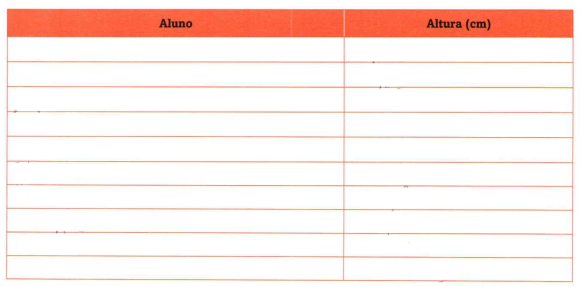
\includegraphics[width=1\linewidth]{6FMA12_imagens/imagem1}
		\begin{itemize}
			\item Soma das alturas de todos os amigos, em centímetros: $\underline{~~~~~~~~~~~~~~~~~~~~~~~~~~~~~~}$.
			\item Média de altura dos amigos da classe: $\underline{~~~~~~~~~~~~~~~~~~~~~~~~~~~~~~}$. \newpage
		\end{itemize}
		\item Faça o mesmo agora com a quantidade de irmãos que cada amigo seu tem: \\
		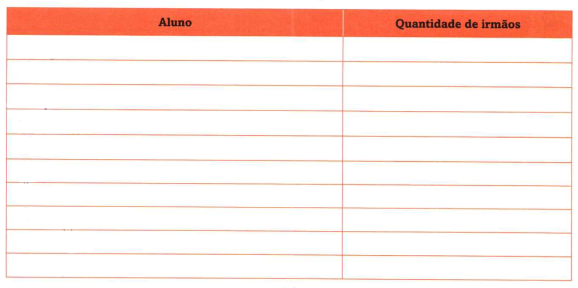
\includegraphics[width=1\linewidth]{6FMA12_imagens/imagem2}
		\begin{itemize}
			\item Soma da quantidade de irmãos dos alunos da classe: $\underline{~~~~~~~~~~~~~~~~~~~~~~~~~~~~~~}$.
			\item Média de irmãos por aluno da classe: $\underline{~~~~~~~~~~~~~~~~~~~~~~~~~~~~~~}$. \newpage
		\end{itemize}
		\item Essa é por sua conta. Decida juntamente com o seu professor um conjunto que possa ser pesquisado dentro da sala e calcule sua média: \\
		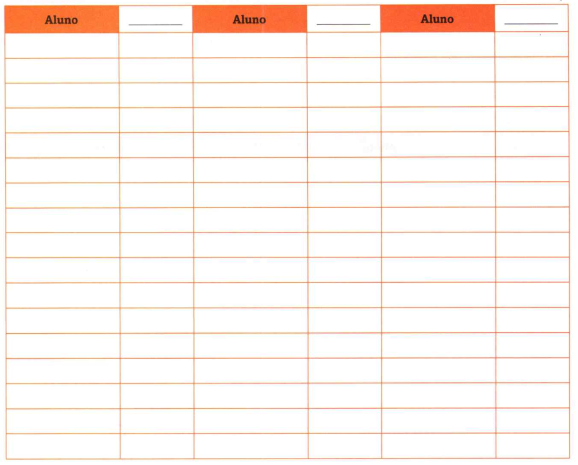
\includegraphics[width=1\linewidth]{6FMA12_imagens/imagem3} \\\\
		\textbf{Desafio olímpico} \\\\
		(OBMEP) Cada uma das figuras está dividida em 16 partes iguais. Em qual delas a parte colorida corresponde a $\frac{5}{8}$ da área total? \\
		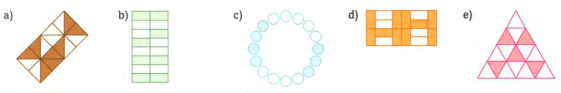
\includegraphics[width=1\linewidth]{6FMA12_imagens/imagem4}
		\newpage
		\item Numa classe com 25 alunos, a prova de Matemática teve 5 notas 10, 6 notas 8, 6 notas 9, 4 notas 7 e 4 notas 5. Calcule a média aritmética das notas dessa prova. \\\\\\\\\\\\\\\\\\\\
		\item Na primeira rodada de um campeonato de futebol, foram marcados 56 gols em 14 jogos. Em média, quantos gols foram marcados por jogo?  \\\\\\\\\\\\\\\\\\\\
		\item Na segunda rodada desse mesmo campeonato de futebol foi registrada uma média de 3 gols por jogo. Quantos gols foram marcados, sabendo que essa rodada teve 6 jogos?  \\\\\\\\\\\\\\\\\\\\
	\end{enumerate}
\end{document}